\chapter{Batch tutorial}
\label{Chap:batch:tutorial}

Details about the algorithms used for data processing are given in the other
sections of this manual. This section explains how a sequence of processing
steps can be run at once without MATLAB programming. SPM8 includes
\texttt{matlabbatch}\footnote{\url{http://sourceforge.net/projects/matlabbatch}}
which has been derived from the SPM5 batch system, but is also available as a
separate package.

In \texttt{matlabbatch}, each data processing step is called ``module''. There
are e.g.\ modules for spatial processing of MRI data (realignment,
normalisation, smoothing), statistics (fMRI or factorial design specification,
model estimation, contrast specification). A batch describes which modules
should be run on what kind of data and how these modules depend on each other.

Compared to running each processing step interactively, batches have a number
of advantages:
\begin{description}
\item[Documentation] Each batch can be saved as a MATLAB script. All
  parameters (including default settings) are included in this script. Thus, a
  saved batch contains a full description of the sequence of processing steps
  and the parameter settings used.
\item[Reproducibility] Batches can be saved, even if not all parameters have
  been set. For a multi-subject study, this allows to create template batches.
  These templates contain all settings which do not vary across subjects. For
  each subject, they can be loaded and only subject-specific parts need to be
  completed.
\item[Unattended execution] Instead of waiting for a processing step to
  complete before entering the results in the next one, all processing steps
  can be run in the specified order without any user interaction.
\item[Multiple batches] Multiple batches can be loaded and executed together.
\end{description}

\section{Single subject}

In this tutorial we will develop a batch for spatial processing and fMRI
statistics of a single subject of the ``Face'' example dataset (see
chapter~\ref{Chap:data:faces}). To follow this tutorial, it is not necessary to
download the example dataset, except for the last step (entering subject
dependent data).

To create a batch which can be re-used for multiple subjects in this study, it
is necessary to collect/define
\begin{itemize}
\item study specific input data (e.g.\ MRI measurement parameters, time
  constants of the functional experiment, number of sessions),
\item necessary processing steps,
\item data flow between processing steps.
\end{itemize}
Subject specific input data (original functional and structural MRI data,
subject specific experiment parameters) should be entered after the batch
template has been saved.

\subsection{Study specific input data}

This dataset consists of fMRI data acquired in a single session and a
structural MRI. See section~\ref{sec:batch_interface_advanced} to learn how to
deal efficiently with multi-session data. MRI parameters and experiment
details are described in chapter~\ref{Chap:data:faces}.

\subsection{Necessary processing steps}

\subsubsection{Helper modules}

Some SPM modules produce graphics output which is captured in a PostScript
file in the current working directory. Also, a new directory needs to be
created for statistics. The ``BasicIO'' menu provides a collection of modules
which are useful to organise a batch. We will need the following modules:

\begin{itemize}
\item Named directory selector
\item Change directory
\item Make directory
\end{itemize}

\subsubsection{SPM processing}

For a classical SPM analysis, the following processing steps are necessary:

\begin{itemize}
\item Realignment
\item Slice timing correction
\item Coregistration
\item Segmentation
\item Normalisation
\item Smoothing
\item fMRI design
\item Model estimation
\item Contrasts
\item Results report
\end{itemize}

\subsection{Add modules to the batch}

The helper modules and the SPM processing modules can be assembled using the
GUI. Click the ``BATCH'' button in the SPM Menu window. First, add the helper
modules, followed by the SPM modules in the order listed above. Do not configure
any details until you have selected all modules.

\begin{figure}
  \centering
  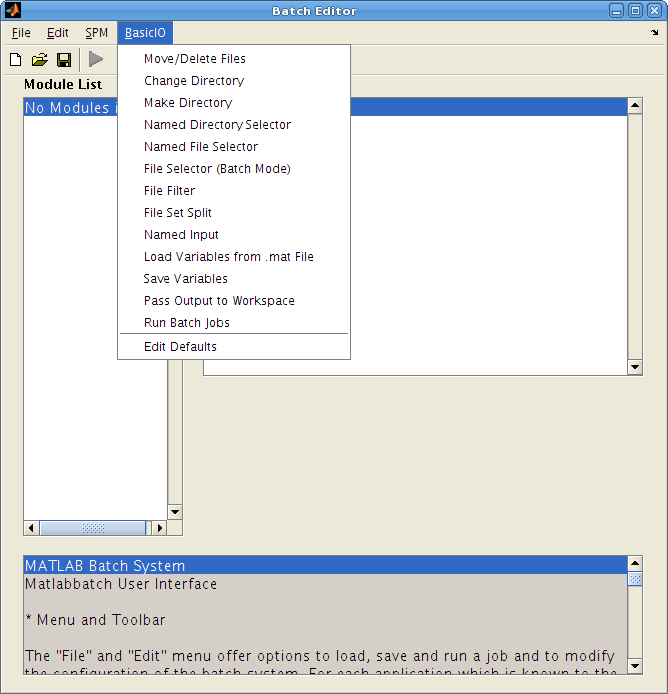
\includegraphics[width=.49\linewidth]{batch/batch_basicio}
  \hfill
  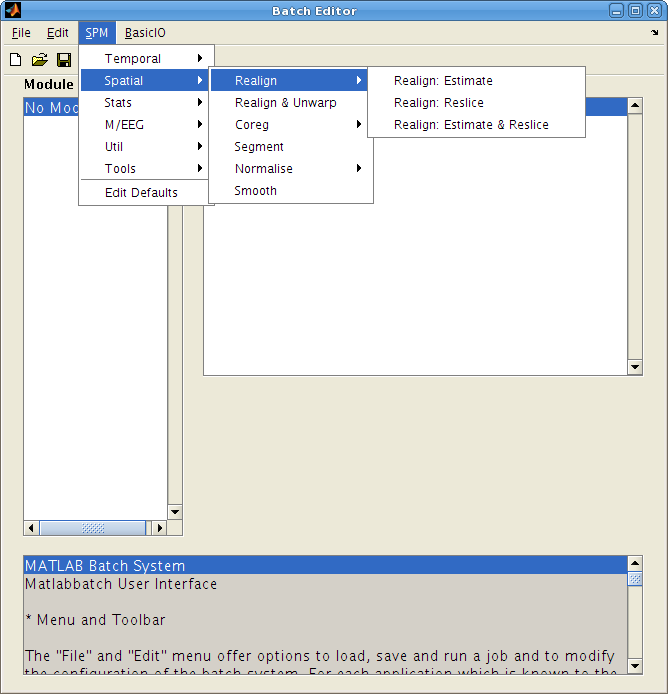
\includegraphics[width=.49\linewidth]{batch/batch_spm}      
  \caption{BasicIO and SPM application menus}
  \label{fig:basicio_spm}
\end{figure}

\subsection{Configure subject-independent data}

Now, go through the batch and configure all settings that are
subject-independent (e.g.\ the name of the analysis directory, slice timing
parameters) as described in chapter~\ref{Chap:data:faces}. Do not enter any data that
is specific for a certain subject. The values that need to be entered are not
repeated here, please refer to the corresponding sections in
chapter~\ref{Chap:data:faces}.

The file \verb|man/batch/face_single_subject_template_nodeps.m| contains the
batch after all modules have been added and subject-independent data has been
entered.

\subsubsection*{Named Directory Selector}

\begin{description}
\item[Input Name] Give this selection a name (e.g. ``Subject directory'') -
  this name will be shown in the dependency list of this batch.
\item[Directories] Add a new directory selector, but do not enter a
  directory itself.
\end{description}

\subsubsection*{Change Directory} 

Nothing to enter now.

\subsubsection*{Make Directory}

\begin{description}
\item[New Directory Name] ``categorical'' - the name of the analysis
  directory. This directory will be created at batch run-time in the subject
  directory. 
\end{description}

\subsubsection*{Realign: Estimate \& Reslice}

\begin{description}
\item[Data] Add a new ``Session'' item. Do not enter any files for this
  session now.
\end{description}

\subsubsection*{Slice Timing}

\begin{description}
\item[Data] Add a new ``Session'' item. Do not enter any files for this
  session now.
\item[Timing options] Enter data for ``Number of slices'', ``TR'', ``TA'',
  ``Slice order'', ``Reference slice''.
\end{description}

\subsubsection*{Coreg: Estimate} 

Nothing to enter now.

\subsubsection*{Segment}

 Nothing to enter now.

\subsubsection*{Normalise: Write}

\begin{description}
\item[Data] Add a new ``Subject''. Do not enter any files now.
\item[Writing Options] Adjust bounding box, voxel sizes, interpolation
\end{description}

\subsubsection*{Smooth}

\begin{description}
\item[FWHM] Enter FWHM
\end{description}

\subsubsection*{fMRI model specification} 

Enter all data which is constant across subjects. 
\begin{description}
\item[Timing parameters] Enter values for ``Units for design'', ``Interscan
  interval'', ``Microtime resolution'', ``Microtime onset''
\item[Data \& Design] Add a new ``Session'' item. Do not enter scans,
  conditions or regressors yet. They will be added as dependencies or
  subject specific inputs. If you want to make sure to remember this, you
  can highlight ``Multiple conditions'' and select ``Clear Value'' from the
  ``Edit'' menu. Do the same for ``Multiple regressors''. This will mark
  both items with an \verb|<-X|, indicating that something must be entered
  there.
\item[Factorial design] Enter the specification for both factors.
\item[Basis functions] Select the basis function and options you want to use.
\end{description}

\subsubsection*{Model estimation}

Nothing to be entered yet for classical estimation.

\subsubsection*{Contrast manager} 

If you have selected the ``Factorial design'' option as described above, SPM
will automatically create some contrasts for you. Here, you can create
additional T- or F-contrasts. As an example, we will add an ``Effects of
interest'' F-contrast. 

\begin{description}
\item[Contrast session] Add a new ``F-contrast'' item.
\item[Name] Enter a name for this contrast, e.g. ``Effects of interest''.
\item[Contrast vectors] Add a new ``Contrast vector'' item. F-contrasts
  can have multiple rows. You can either enter a contrast matrix in an ``F
  contrast vector'' entry, or enter them row by row. To test for the
  effects of interest (1 basis function and 2 derivatives for each of the
  four conditions) enter \verb|eye(12)| as F contrast vector.
\item[Replicate over sessions] This design does not have multiple
  sessions, so it is safe to say ``No'' here.
\end{description}

\subsubsection*{Results report}

Reviewing individual results for a large number of subjects can be very time
consuming. Results report will print results from selected contrasts to a
PostScript file. 
  
\begin{description}
\item[Contrast(s)] Enter \verb|Inf| to print a report for each of the
  defined contrasts.
\end{description}

\subsection{Data flow}

In chapter~\ref{Chap:data:faces}, each processing step was performed on its own. In
most cases, output data was simply passed on from one module to the next. This
scheme is illustrated in figure~\ref{fig:flow}. Only the coloured items at the
top of the flow chart are subject specific and need to be entered in the final
batch. All arrow connections are subject-independent and can be specified in
the batch template.

\begin{figure}
  \centering
  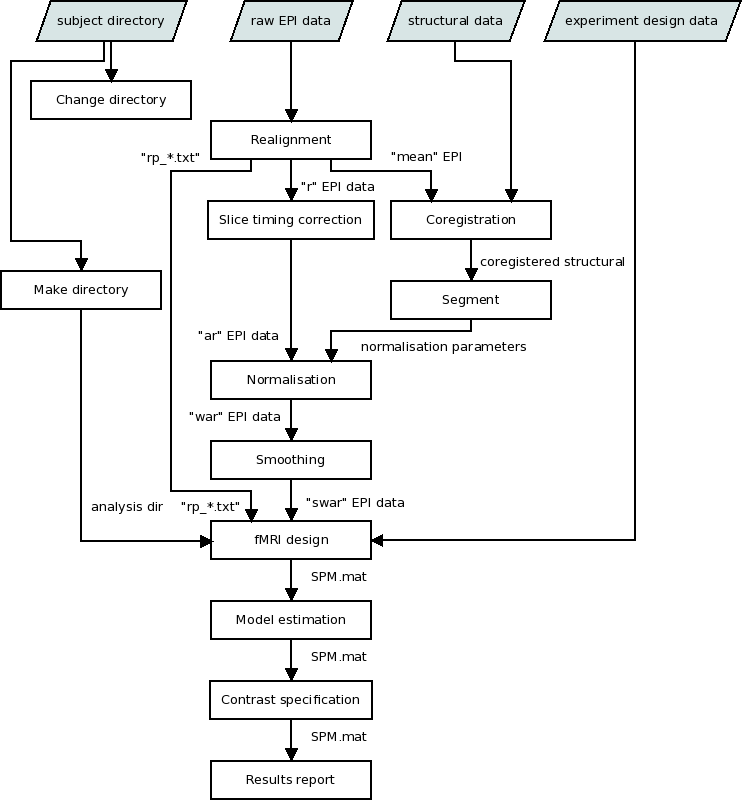
\includegraphics[width=.9\linewidth]{batch/flow}
  \caption{Flow chart for batch}
  \label{fig:flow}
\end{figure}

\subsubsection{Add dependencies}

Based on the data flow in figure~\ref{fig:flow}, modules in the batch can now
be connected. The batch containing all dependencies can be found in
\verb|man/batch/face_single_subject_template.m|.

\begin{figure}[htbp]
  \centering
  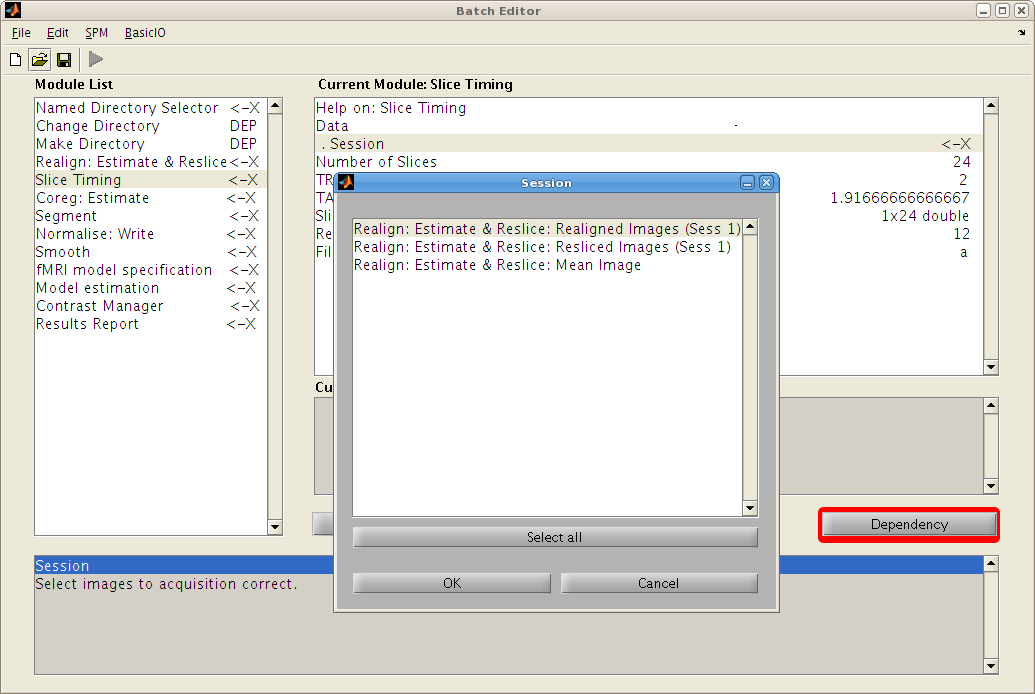
\includegraphics[width=\textwidth]{batch/batch_dependencies}
  \caption{Dependency selection}
  \label{fig:batch_dependency}
\end{figure}

Again, start editing at the top of the batch:

\subsubsection*{Named Directory Selector}

Nothing to enter now.

\subsubsection*{Change Directory}

\begin{description}
\item[Directory] Press ``Dependency'' and select ``Subject
  directory(1)''. At run time, SPM will change to this directory before batch
  processing continues.
\end{description}

\subsubsection*{Make Directory}

\begin{description}
\item[Parent Directory] Press ``Dependency'' and select ``Subject
  directory(1)''. The ``categorial'' directory will be created in this
  directory. 
\end{description}

\subsubsection*{Realign: Estimate \& Reslice}

Nothing to enter now.

\subsubsection*{Slice Timing}

\begin{description}
\item[Session] Press ``Dependency'' and select ``Resliced Images (Sess~1)''.
\end{description}

\subsubsection*{Coreg: Estimate}

\begin{description}
\item[Reference Image] Press ``Dependency'' and select ``Mean Image''.
\end{description}

\subsubsection*{Segment}

\begin{description}
\item[Data] Press ``Dependency'' and select ``Coregistered Images''. At run
  time, this will resolve to the coregistered anatomical image.
\end{description}

\subsubsection*{Normalise: Write}

\begin{description}
\item[Parameter File] Press ``Dependency'' and select ``Norm Params File
  Subj$\rightarrow$MNI (Subj~1)''.
\item[Images to Write] Press ``Dependency'' and select ``Slice Timing
  Corr. Images (Sess~1)''. 
\end{description}

\subsubsection*{Smooth}

\begin{description}
\item[Images to Smooth] Press ``Dependency'' and select ``Normalised Images
  (Subj~1)''
\end{description}

\subsubsection*{fMRI model specification}

\begin{description}
\item[Directory] Press ``Dependency'' and select ``Make Directory
  'categorical'\,''
\item[Scans] Press ``Dependency'' and select ``Smoothed Images''. Note: this
  works because there is only one session in our experiment. In a
  multisession experiments, images from each session may be normalised and
  smoothed using the same parameters, but the smoothed images need to be
  split into sessions again. See section~\ref{sec:batch_interface_advanced}
  how this can be done.
\item[Multiple regressors] Press ``Dependency'' and select ``Realignment
  Param File (Sess~1)''.
\end{description}

\subsubsection*{Model estimation}

\begin{description}
\item[Select SPM.mat] Press ``Dependency'' and select ``SPM.mat File (fMRI
  Design\&Data)''.
\end{description}

\subsubsection*{Contrast manager}

\begin{description}
\item[Select SPM.mat] Press ``Dependency'' and select ``SPM.mat File
  (Estimation)''. 
\end{description}

\subsubsection*{Results report}

\begin{description}
\item[Select SPM.mat] Press ``Dependency'' and select ``SPM.mat File
  (Contrasts)''. 
\end{description}

\subsection{Entering subject-specific data}

Now, only 4 modules should have open inputs left (marked with \verb|<-X|). These
inputs correspond to data which vary over the subjects in your study:
\begin{description}
\item[Named Directory Selector] Subject directory
\item[Realign: Estimate \& Reslice] Raw EPI data for the fMRT session
\item[Coreg: Estimate] Anatomical image to be coregistered to mean EPI
\item[fMRI model specification] Names, conditions and onsets of your
  experimental conditions, specified in a multiple conditions .mat file.
\end{description}

Using the GUI, you can now perform these steps for each subject:
\begin{enumerate}
\item load the template batch
\item enter subject-specific data
\item save batch under a subject specific name.
\end{enumerate}

After that, all batches for all subjects can be loaded and run at once.

This process can be automated using some basic MATLAB scripting. See
section~\ref{sec:batch_interface_cmd_cfg_serial} for details.

\begin{figure}[htbp]
  \centering
  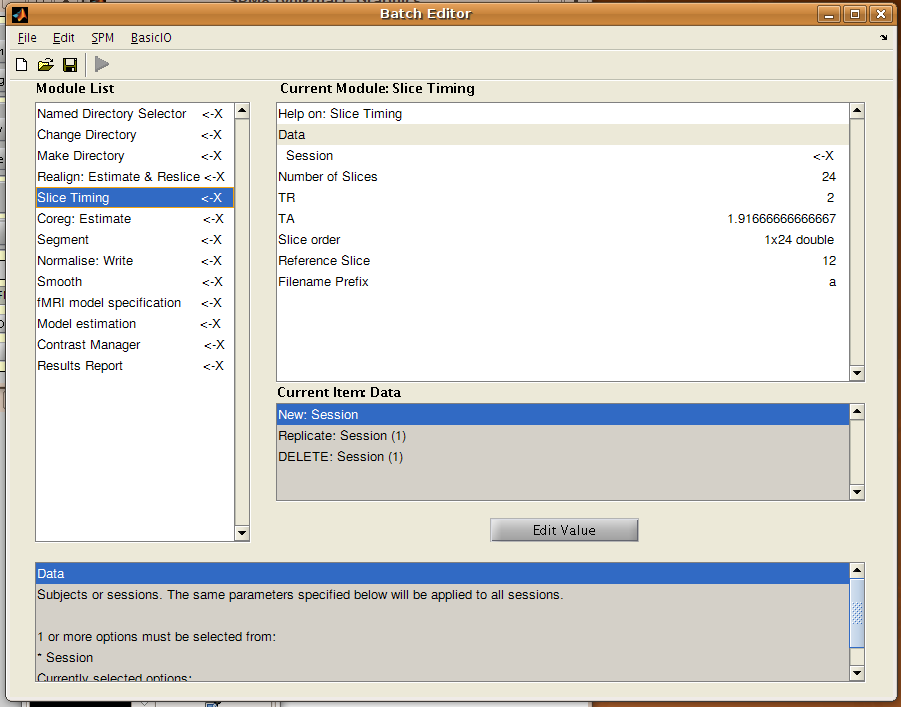
\includegraphics[height=.3\textheight]{batch/batch_single_subject_template_nodeps}

  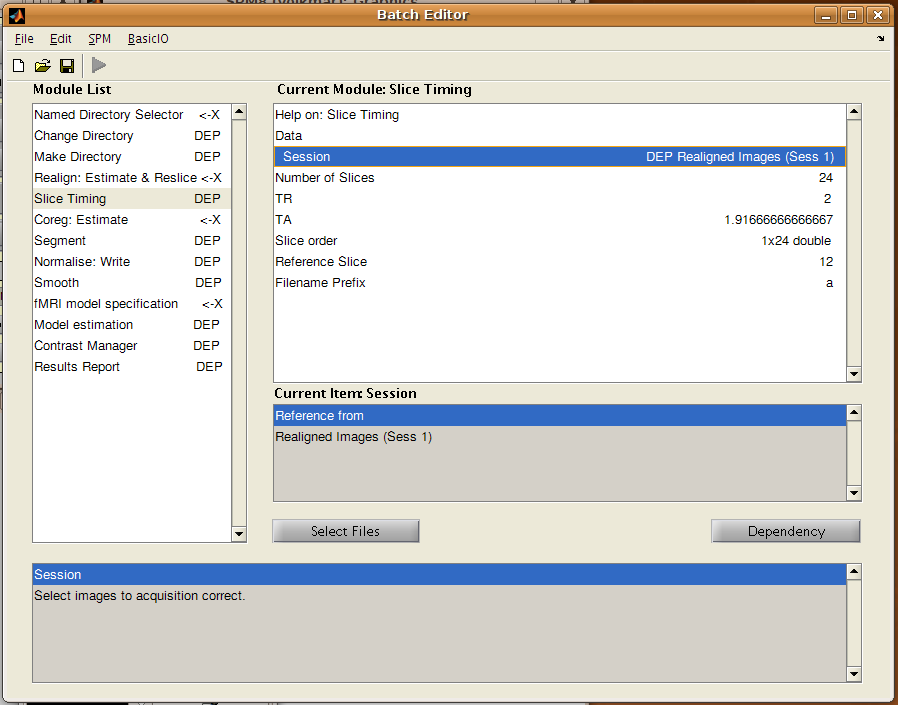
\includegraphics[height=.3\textheight]{batch/batch_single_subject_template}

  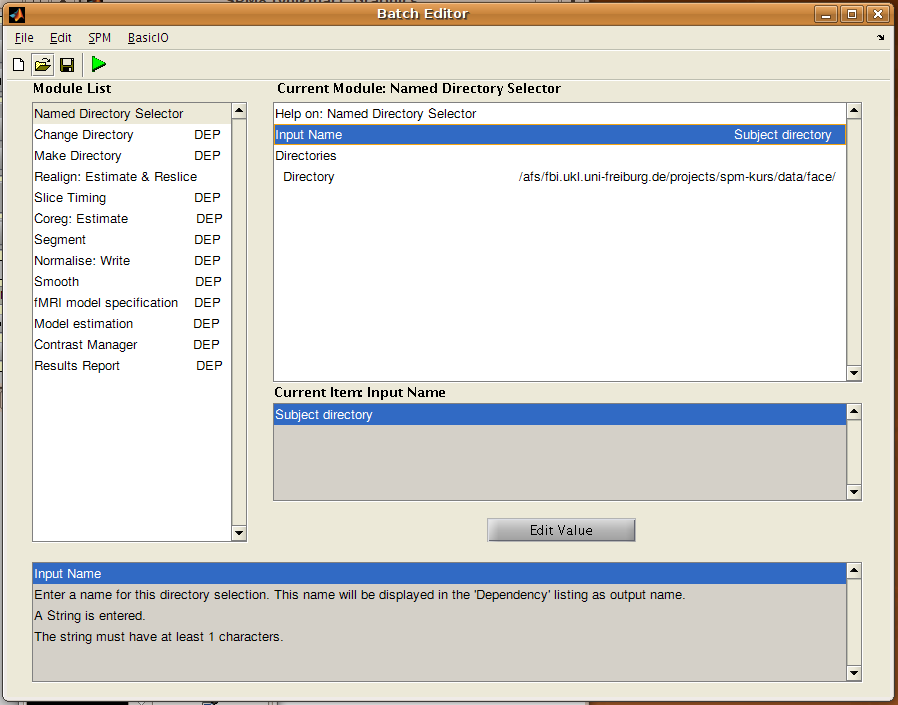
\includegraphics[height=.3\textheight]{batch/batch_single_subject}

  \caption{All stages of batch entry}
  \label{fig:batch_stages}
\end{figure}

\section{Advanced features}
\label{sec:batch_interface_advanced}

\subsection{Multiple sessions}

If an fMRI experiment has multiple sessions, some processing steps need to
take this into account (slice timing correction, realignment, fMRI design),
while others can work on all sessions at once (normalisation, smoothing). 

Two modules in BasicIO help to solve this problem:
\begin{description}
\item[Named File Selector] Files can be entered here session by session. Note
  that this file selector selects all files (not restricted to images) by
  default. To select only images, set the filter string to something like
  \verb|.*nii$| or \verb|.*img$|.
\item[File Set Split] This module splits a list of files based on an index
  vector. Named file selector provides such an index vector to split the
  concatenation of all selected images into individual sessions again.
\end{description}

\subsection{Processing multiple subjects in GUI}

There are different ways to process multiple subjects in the batch
editor:
\begin{itemize}
\item Add the necessary processing steps when creating the job.
\item Create a per-subject template, save it and load it multiple
  times (i.e. in the file selector, add the same file multiple times
  to the list of selected files).
\item Use ``Run Batch Jobs'' from ``BasicIO''
\end{itemize}

\begin{figure}[htbp]
  \centering
  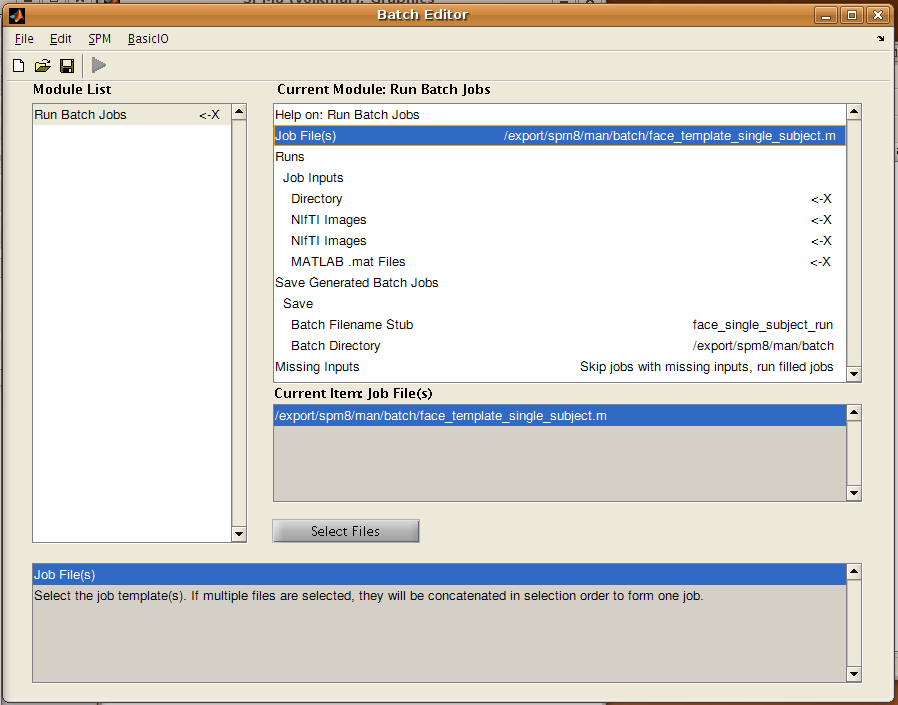
\includegraphics[width=.9\linewidth]{batch/batch_multi_subject_template}

  \caption{Using ``Run Batch Jobs''}
  \label{fig:batch_multi_subject_template}
\end{figure}

In all cases, the data for all subjects has to be entered through the
GUI, and computation will be done for all subjects at once after all
data is entered. There is an example job
\verb|face_multi_subject_template.m| that demonstrates the usage of
``Run Batch Jobs'' to run the single subject template job described
above. Note that the order and type of inputs in the single subject
template is important. Also, consistency checks are limited. If
inconsistent data is entered, the job will fail to execute and return
an error message.

To run this job for multiple subjects, simply repeat the ``Runs'' item
as many times as necessary and fill in the required data.

\subsection{Command line interface}
\label{sec:batch_interface_cmd}

The command line interface is especially useful to run multiple jobs
at once without user interaction, e.g.\ to process multiple subjects
or to combine separate processing steps. There is a ``high-level''
interface using \verb|spm_jobman|, which combines ``low-level''
callbacks to \verb|cfg_util|.

\subsubsection{SPM startup in command line mode}
\label{sec:batch_interface_spm_startup}

During normal startup, SPM performs important initialisation
steps. Without initialisation, SPM and its batch system will not
function properly. Consequently, an initialisation sequence needs to
be run before any batch job can be submitted.

MATLAB has several command line options to start without its GUI
(\verb|-nodesktop|) or even without any graphics output to a screen
(\verb|-nodisplay|). See MATLAB documentation for details.

To run SPM in \verb|-nodisplay| mode, the file \verb|spm_defaults.m|
has to be modified. The line \verb|defaults.cmdline = 0;| must be
changed to \verb|defaults.cmdline = true;|. In command line mode, SPM
will not open any figure window except the ``Graphics'' window. 

Within MATLAB, the following commands are sufficient to set up SPM
\begin{enumerate}
\item \verb|spm('defaults', MODALITY)| where \verb|MODALITY| has to be
  replaced by the desired modality (e.g. \verb|'fmri'|)
\item \verb|spm_jobman('initcfg')|
\end{enumerate}
After executing these commands, any SPM functions and batch jobs
can be run in the same MATLAB session.

\subsubsection{Complete and run a pre-specified job}
\label{sec:batch_interface_cmd_cfg_serial}

\verb|spm_jobman('serial', job[,'', input1, input2 ...])|

This interface is called the ``serial'' interface. It takes a job, and asks
for the input to any open configuration items one after another. If a list of
inputs is supplied, these will be filled in (if they are appropriate). After
all inputs are filled, the job will be run. Note that only items 
without a pre-set value will be filled (marked with \verb|<-X| in
the GUI). To force a item to to be filled, use ``Edit:Clear Value''
in the GUI or set its value to \verb|'<UNDEFINED>'| in the harvested job.

The job argument is very flexible, it can e.g.\ be a job variable, the
name of a script creating a job variable, even a cell list of any
mixture of variables and scripts. All job snippets found will be
concatenated into a single job, the missing inputs will be filled and
the resulting job will be run.

The batch system can generate a script skeleton for any loaded
job. From the batch GUI, this feature is accessible via ``File:Save
Batch and Script''. This skeleton consists of a commented list of
necessary inputs, a \verb|for| loop to enter inputs for multiple runs
or subjects and the code to initialise and run the job. An example is
available in \verb|face_single_subject_script.m|:

\begin{verbatim}
% List of open inputs
% Named Directory Selector: Directory - cfg_files
% Realign: Estimate & Reslice: Session - cfg_files
% Coreg: Estimate: Source Image - cfg_files
% fMRI model specification: Multiple conditions - cfg_files
nrun = X; % enter the number of runs here
jobfile = {fullfile(spm('dir'),'man','batch','face_single_subject_template.m')};
jobs = repmat(jobfile, 1, nrun);
inputs = cell(4, nrun);
for crun = 1:nrun
    % Named Directory Selector: Directory - cfg_files
    inputs{1, crun} = MATLAB_CODE_TO_FILL_INPUT;
    % Realign: Estimate & Reslice: Session - cfg_files
    inputs{2, crun} = MATLAB_CODE_TO_FILL_INPUT; 
    % Coreg: Estimate: Source Image - cfg_files
    inputs{3, crun} = MATLAB_CODE_TO_FILL_INPUT; 
    % fMRI model specification: Multiple conditions - cfg_files
    inputs{4, crun} = MATLAB_CODE_TO_FILL_INPUT; 
end
spm('defaults','fmri');
spm_jobman('serial',jobs,'',inputs{:});
\end{verbatim}

The skeleton needs to be adapted to the actual data layout by adding
MATLAB code which specifies the number of runs and the input data in
the \verb|for| loop.

Another example script and batch is available for the multimodal
dataset, called \verb|multimodal_fmri_script.m| and
\verb|multimodal_fmri_template.m|.

\subsection{Modifying a saved job}

In some cases, instead of using the serial interface it may be more
appropriate to modify the fields of a saved or harvested job. By default, jobs
are saved as MATLAB \verb|.mat| files, but they can also be saved as
\verb|.m| files. These files contain a number of MATLAB commands,
which will create a variable \verb|matlabbatch|. The commands can be
modified to set different values, add or remove options. 
